\chapter{Résultats et perspectives}

\section{Résultats et difficultés rencontrées}

\subsection*{Résultats}


Nous sommes donc capables, étant donné un complexe stocké dans un fichier \textit{.pdb},
d'afficher ce complexe (voir figure \ref{fig::complexe}) et de visualiser la surface
de contact dans Meshlab (voir figure \ref{fig::affichage_final}).

\begin{figure}[ht]
\centering
  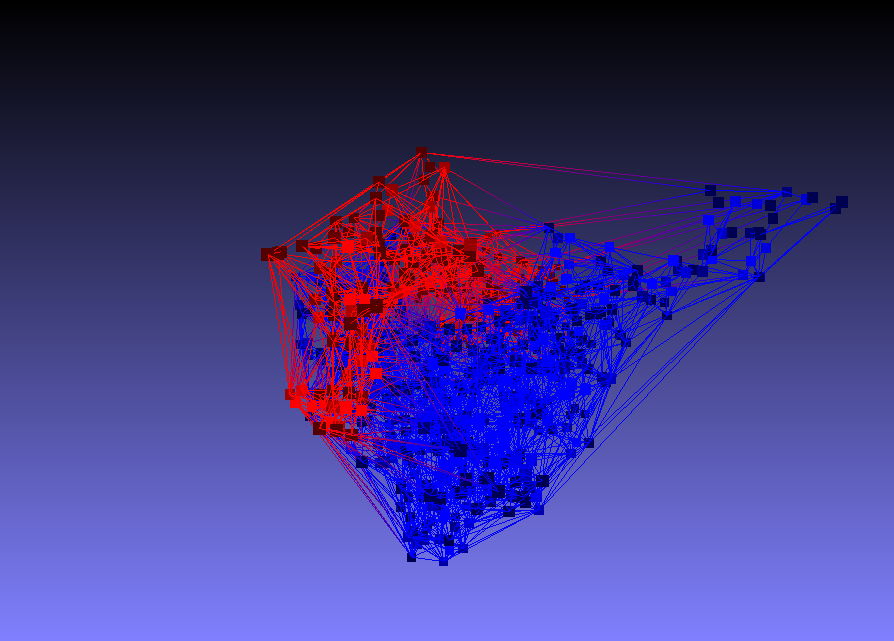
\includegraphics[width=0.8\textwidth]{figures/final_no_surf.png}
  \caption{Complexe}
  \label{fig::complexe}
\end{figure}

\begin{figure}[ht]
\centering
  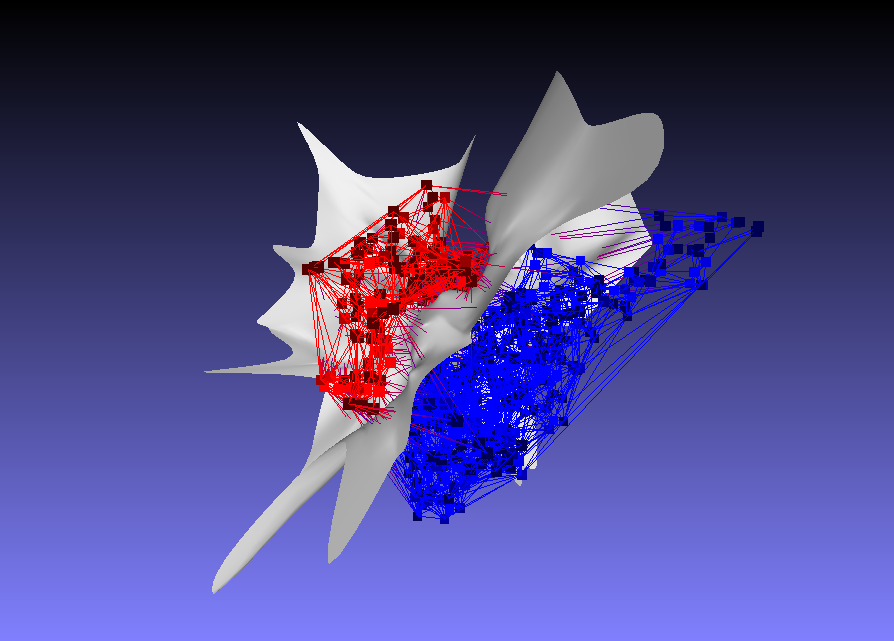
\includegraphics[width=0.8\textwidth]{figures/final_with_surf.png}
  \caption{Affichage de l'interface entre deux protéines}
  \label{fig::affichage_final}
\end{figure}

La méthode d'indexation permet de connaître à tout moment les particularités de chaque
atome et de lier ces informations à la surface. Les deux atomes formant une arête
de l'interface correspondent à un morceau de la surface. Il est donc possible, par exemple,
de colorer la surface en fonction du type de l'atome qui lui correspond ou de l'acide aminé
auquel celui-ci appartient.

La visualisation dans MeshLab permet de bien comprendre comment les protéines du complexe interagissent.
Deux types de visualisation de la surface sont possibles :
\begin{itemize}
  \item sans lissage (voir figure \ref{fig::surf_no_smooth}) : les morceaux de la surface correspondent
  directement aux duaux de chaque arête
  \item avec lissage (voir figure \ref{fig::surf_smooth}) : le lissage de la surface
  permet d'obtenir une surface continue lors de l'affichage.
\end{itemize}

\begin{figure}[ht]
\centering
  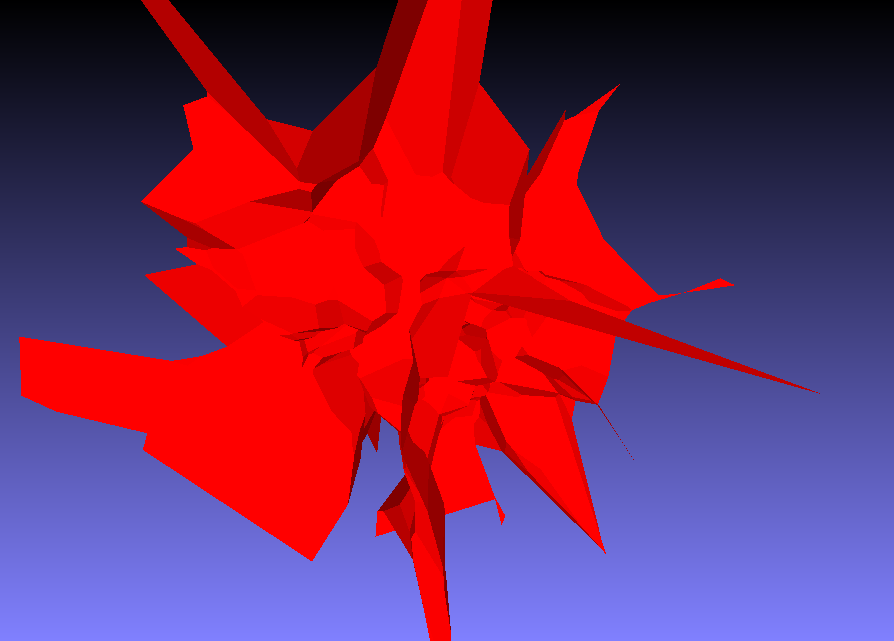
\includegraphics[width=0.8\textwidth]{figures/surf_no_smooth.png}
  \caption{Affichage de l'interface non lissée}
  \label{fig::surf_no_smooth}
\end{figure}

\begin{figure}[ht]
\centering
  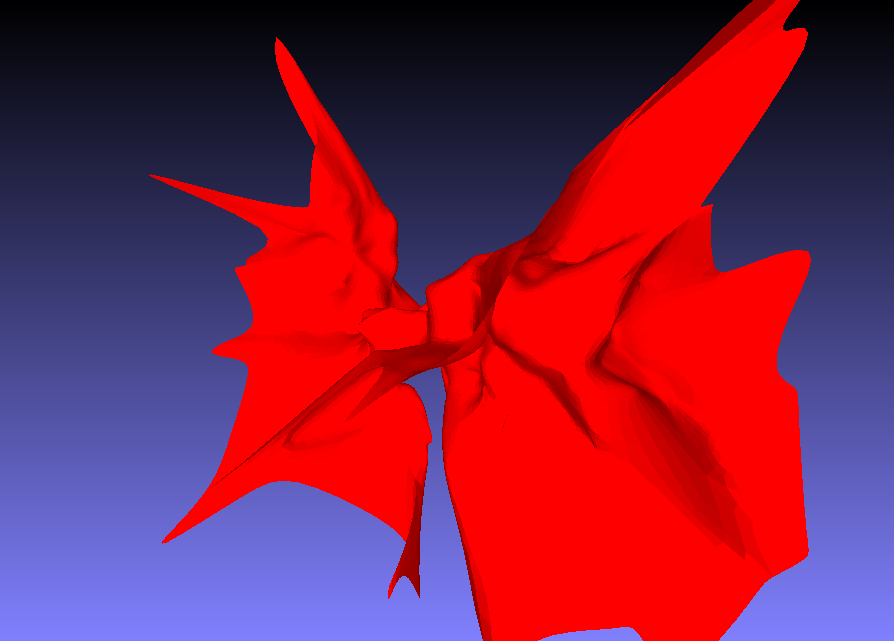
\includegraphics[width=0.8\textwidth]{figures/surf_smooth.png}
  \caption{Affichage de l'interface lissée}
  \label{fig::surf_smooth}
\end{figure}

Finalement, l'objectif principal, qui était d'afficher un complexe protéique avec son
interface de contact sous forme d'une surface lisse en trois dimensions a été rempli.
Cependant, nous avons, pour arriver à ce résultat, rencontré un certain nombre de difficultés que nous
détaillons dans la partie suivante.


\subsection*{Difficultés rencontrées}
Les deux difficultés principales auxquelles nous avons été confrontés au long de ce projet
sont les suivantes :
\begin{itemize}
  \item comment compiler le projet sachant qu'il regroupe différentes méthodes d'implémentation
  \item l'utilisation de \gls{cgal} qui bien qu'efficace peut parfois se montrer rigide
\end{itemize}

Ainsi, la compilation du projet s'est trouvée compliquée par le fait que \gls{cgal} peut être difficile
à intégrer à un projet de grande envergure. En effet, la documentation permet de
comprendre facilement comment compiler un petit projet utilisant \gls{cgal}. En revanche, l'utilisation de Cmake
pour rassembler les différentes partie peut être laborieuse. Ainsi, compiler un tel projet
requiert de maîtriser la méthode de compilation par Cmake. Cela permet également de comprendre
que le développement d'un tel projet, en partant de rien, suppose de maîtriser différentes
méthodes de compilation.

Ensuite, \gls{cgal} est destiné à un utilisateur expert et se trouve être difficile à prendre
en main pour un utilisateur novice. En effet, il est absolument nécessaire, avant de
démarrer l'implémentation d'un projet, d'être familier avec les structures fournies par \gls{cgal}.
Etant donnée la taille de \gls{cgal}, on comprend aisément qu'un temps important doit être
consacré à cela. Ceci pouvant finalement faire perdre du temps par rapport à l'utilisation de méthodes
et de structures personnelles. En revanche, une fois prise en main, il est important de souligner la puissance
de calcul et l'aide au développement que fournit \gls{cgal}.

Pour illustrer ceci, il est important de replacer le projet dans son contexte. Nous avons
choisi, au départ, d'utiliser au maximum les fonctionnalités fournies par \gls{cgal}.
Dans cette optique, j'ai perdu un temps conséquent à vouloir toujours fonctionner de cette manière.
CGAL fournit en effet nombre de structures (\textit{vector}, \textit{map}) semblables
à celles présentes dans la bibliothèque standard (\textit{std}) du C++. En revanche, l'utilisation
de cette dernière est plus simple car nous sommes déjà familiers de sa méthode de fonctionnement.
Ainsi, nous avons choisi de revenir à des structures connues. Par exemple, pour le stockage de la
surface, seules les classes de la bibliothèque standard sont utilisées, ce qui s'est
révélé être le choix le plus efficace.

L'objectif ici n'est pas d'infirmer la puissance de calcul offerte par \gls{cgal} ou son utilité.
L'utilisation de la triangulation de Delaunay aurait été beaucoup plus difficile
à implémenter sans cette bibliothèque. Il semble simplement important de préciser qu'il peut être
parfois plus efficace de développer certaines méthodes en se passant d'une bibilothèque extérieure.
Ainsi les structures créées directement par le développeur ont l'avantage d'être
parfaitement connues et donc plus efficaces dans certains cas.

\section{Perspectives}

La méthode d'affichage utilisée (indexation des points et affichage par triangles)
peut permettre de passer facilement en OpenGL. En effet, OpenGL fonctionne par l'affichage
de triangles dont les indices renvoient à une liste de points stockée auparavant.
Etant donnée la méthode utilisée pour afficher le complexe et son interface, il semble
raisonnable d'affirmer que cela est tout à fait possible dans le cadre de ce projet.
Un affichage via OpenGL permettrait par exemple d'obtenir un meilleur rendu que sur
MeshLab car les possibilités sont plus nombreuses.

De plus, l'un des objectifs du projet est de modifier dynamiquement la surface de contact
en fonction des mouvements des atomes de la protéines. Le complexe peut changer de structure
avec des mouvements, voire des ajouts et des suppression d'atomes. La méthode aurait été
de recalculer par endroits (en fonction des modifications) la triangulation de Delaunay.
Grâce au structures fournies par \gls{cgal}, il est possible d'ajouter ou de supprimer
un point dans une triangulation sans la recalculer entièrement. Un déplacement d'atome
revient à une suppression puis un ajout en conservant l'indice. En utilisant des fichiers \textit{.pdb}
fournissant différents états d'un complexe, nous aurions voulu implémenter une méthode
permettant d'afficher la surface à chacun de ces états. La problématique principale
aurait été d'optimiser le temps de calcul pour permettre au programme de calculer un maximum
d'états différents. L'observation dynamique est effet intéressante car elle permet d'analyser
les déformations de la surface en fonction des mouvements des atomes.

Toujours dans cette optique dynamique, l'utilisation d'OpenGL aurait été recommandée.
En effet, on peut imaginer une visualisation des différents états en une seule fois (sous
forme de vidéo par exemple). Dans ce cas, la génération d'un fichier \textit{.off}
semble trop lourde et probablement trop lente. La conservation des différents états de
la surface n'est pas forcément nécessaire.

De plus, on peut exploiter la surface obtenue en affichant des informations sur
les atomes. Par exemple, il serait possible de colorer la surface en fonction des propriétés
des atomes (poids, liaison, acide aminé, etc.). Cela permettrait d'analyser plus facilement
la surface. Il serait alors intéressant de projeter la surface en deux dimensions afin
de comparer les complexes par superposition.

Finalement, grâce à l'architecture choisie pour le projet, il est possible de le
modifier assez simplement dans le but d'ajouter des fonctionnalités.
